\section{Experimental Results and Discussion}

\subsection{Experimental Setup}

All experiments were conducted using Python and standard machine learning and deep learning libraries. The dataset was divided into training, validation, and testing sets using a stratified 70:15:15 split to ensure balanced class distributions across all subsets.

Three classification approaches were evaluated:

\begin{enumerate}
\item ORB feature extraction with Bag-of-Visual-Words (BoVW) representation and traditional machine learning classifiers.
\item A custom Convolutional Neural Network (CNN) trained from scratch.
\item A MobileNetV2 transfer learning model initialized with ImageNet pre-trained weights.
\end{enumerate}

Performance was measured using classification accuracy on both validation and test datasets. The validation set was used for model selection and hyperparameter tuning, while the test set was reserved for final performance evaluation.

\subsection{Dataset Summary}

After preprocessing and quality filtering, the final dataset contained 425 images distributed across 14 herbal plant classes. The preprocessing pipeline removed low-quality images affected by excessive blur and insufficient vegetation coverage.

% Table 2: Dataset distribution by class

The dataset as shown in \cref{tab:dataset_stats} presents a challenging classification problem due to variations in lighting conditions, viewing angles, background clutter, and intra-class appearance differences.

\subsection{Performance of Traditional Machine Learning Models}

The first set of experiments evaluated traditional machine learning algorithms using ORB descriptors and Bag-of-Visual-Words representations.

Table~\ref{tab:traditional_results} summarizes the validation performance of the evaluated classifiers.

\begin{table}[t]
\centering
\caption{Traditional classifier validation results on the preprocessed plant dataset.}
\label{tab:traditional_results}
\begin{tabular}{lc}
\toprule
\textbf{Model} & \textbf{Validation Accuracy (\%)} \\
\midrule
SVM                 & \textbf{47.92} \\
Logistic Regression & 45.83 \\
Random Forest       & 31.77 \\
Gradient Boosting   & 28.65 \\
\bottomrule
\end{tabular}
\end{table}

Among the evaluated models, the Support Vector Machine (SVM) achieved the highest validation accuracy of 47.92\%, outperforming Random Forest, Logistic Regression, and Gradient Boosting classifiers. Consequently, the SVM model was selected for final testing.

When evaluated on the unseen test set, the ORB-BoVW-SVM pipeline achieved a test accuracy of 36.46\%. Although the model successfully captured local texture and shape information, its performance was limited by the handcrafted nature of the extracted features. The Bag-of-Visual-Words representation also discards spatial relationships between image regions, which can be important for distinguishing visually similar plant species.

\subsection{Performance of the Custom CNN}

A custom Convolutional Neural Network was trained from scratch using the herbal plant dataset. Despite its ability to learn hierarchical feature representations directly from image data, the model achieved a test accuracy of only 22.40\%.

% Figure 8: CNN training and validation accuracy curves
% Figure 9: CNN training and validation loss curves
\begin{figure*}[t]
  \centering
  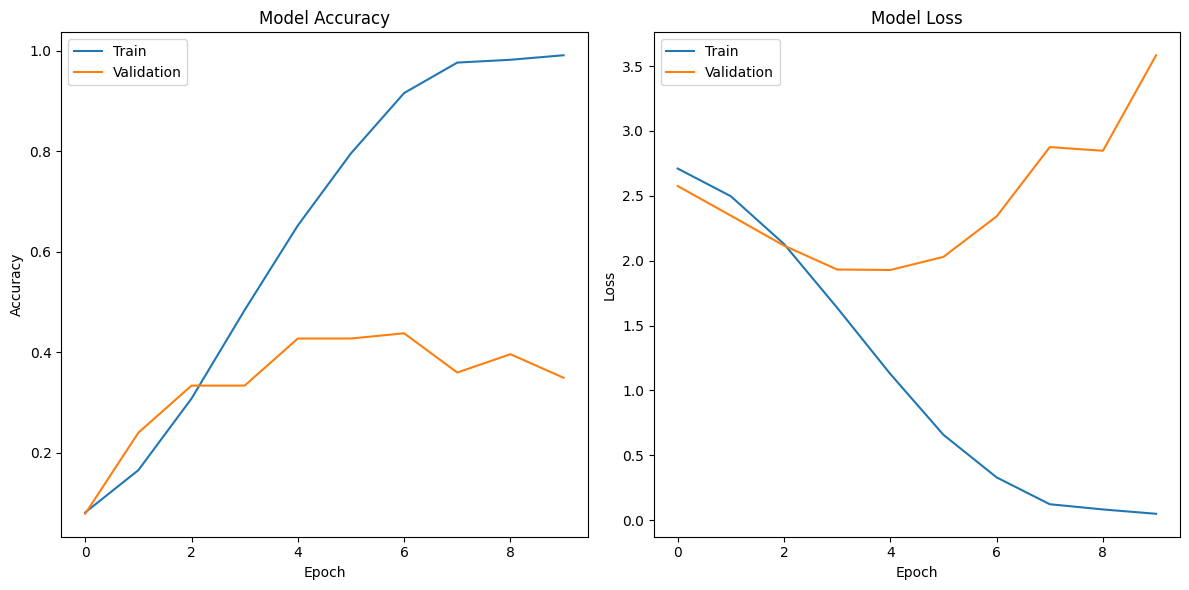
\includegraphics[width=0.95\linewidth]{media/cnn-curves.png}
  \caption{CNN training and validation loss curves}
  \label{fig:cnncurves}
\end{figure*}


As shown in \cref{fig:cnncurves}, the relatively poor performance can largely be attributed to the limited size of the training dataset. Deep neural networks typically require large numbers of labeled examples to learn robust and generalizable feature representations. With only 425 images distributed across 14 classes, the network likely struggled to learn discriminative features while avoiding overfitting.

Furthermore, plant classification represents a fine-grained recognition task where subtle differences between species must be captured. A shallow custom CNN trained from scratch may not possess sufficient representational capacity to learn these distinctions effectively from a small dataset.

\subsection{Performance of MobileNetV2 Transfer Learning}

The transfer learning approach based on MobileNetV2 produced the best performance among all evaluated methods. The model achieved a test accuracy of 93.23\%, substantially outperforming both the traditional machine learning pipeline and the custom CNN.

% Figure 10: MobileNetV2 training and validation accuracy curves

% Figure 11: MobileNetV2 training and validation loss curves


The strong performance of MobileNetV2 can be attributed to its pre-trained feature extraction capabilities. Since the network was initially trained on the large-scale ImageNet dataset, it had already learned rich visual representations useful for recognizing textures, shapes, edges, and object structures. Fine-tuning these representations for herbal plant classification required significantly less training data than learning features from scratch.

Additionally, MobileNetV2 employs depthwise separable convolutions, allowing efficient feature extraction while maintaining strong classification performance. This architecture proved particularly suitable for the relatively small and diverse dataset used in this study.

\subsection{Comparative Analysis}

Table~\ref{tab:comparison_results} presents the final comparison of all evaluated approaches.

% Table 4: Final model comparison
\begin{table}[t]
\centering
\caption{Final model comparison evaluated on the test set.}
\label{tab:comparison_results}
\begin{tabular}{lc}
\toprule
\textbf{Method} & \textbf{Test Accuracy (\%)} \\
\midrule
MobileNetV2   & \textbf{93.23} \\
SVC  & 36.46 \\
Custom CNN    & 22.40 \\
\bottomrule
\end{tabular}
\end{table}

The results in \cref{tab:comparison_results} demonstrate a clear performance hierarchy among the evaluated methods. Traditional feature-based approaches achieved moderate performance by leveraging local image descriptors and machine learning classifiers. However, handcrafted features were unable to fully capture the complex visual characteristics required for reliable plant classification.

Interestingly, the custom CNN performed worse than the traditional ORB-BoVW-SVM pipeline. This result highlights an important challenge in deep learning: training neural networks from scratch with limited data often leads to poor generalization. While CNNs possess greater representational power than handcrafted features, their effectiveness depends heavily on the availability of sufficient training examples.

The MobileNetV2 transfer learning approach achieved the highest classification accuracy by a large margin. Compared to the ORB-BoVW-SVM pipeline, MobileNetV2 improved test accuracy by approximately 56.77 percentage points. Compared to the custom CNN, the improvement was approximately 70.83 percentage points.

These findings demonstrate that transfer learning provides a highly effective solution for plant recognition tasks where dataset size is limited. The ability to leverage previously learned visual representations allows deep learning models to achieve excellent performance without requiring extensive data collection efforts.

% Figure 12: Confusion matrix for MobileNetV2

% Figure 13: Sample correct and incorrect classifications

\subsection{Limitations}

Several limitations should be considered when interpreting the results. First, the dataset contains only 425 images, which may not fully represent the visual diversity of herbal plant species encountered in real-world environments. Second, the dataset was derived from only 21 video sequences, potentially limiting environmental variability.

Additionally, only image-based classification was investigated. Future work could explore object detection, segmentation, multimodal approaches, or larger datasets containing additional plant species and environmental conditions.

Despite these limitations, the results demonstrate the feasibility of automated herbal plant classification and highlight the effectiveness of transfer learning for practical plant recognition applications.
